% \chapter{Search spaces}

\newpage

Before going further with our quest for efficient RL. Let's explore some
properties of our chosen setting, MDPs.


\section{The value function polytope}

The value function polytope \cite{Dadashi2018} provides some great intuition
about the structure of a MDP and the dynamics of optimisation. Let's take a look.

\begin{figure}
\centering
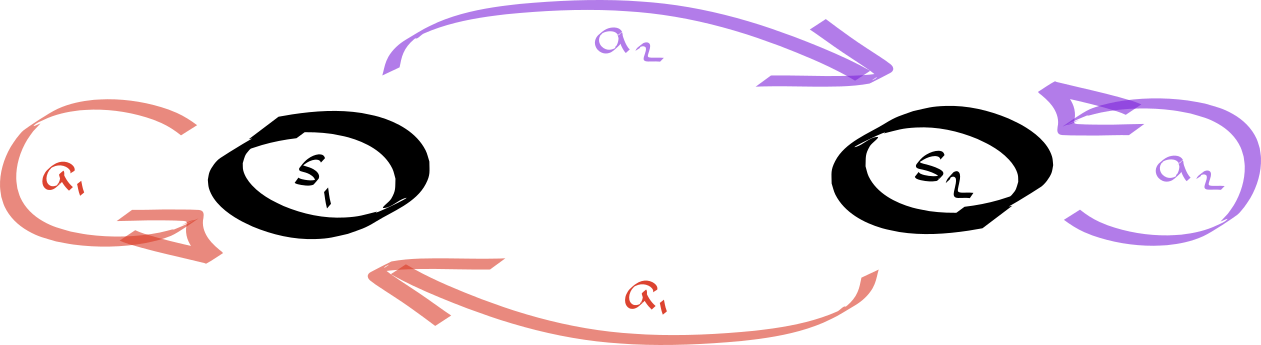
\includegraphics[width=1\textwidth,height=0.25\textheight]{../../pictures/drawings/2-state-automata.png}
\caption{Consider the simplest possible MDP, with two states and two actions. (Any simpler setting is entierly uninteresting. A single state means actions do nothing.
And a single action means all policies are the same.).}
\end{figure}

Consider a two state MDP. The space of possible policies is a 2D space
consisting of action 1 and action 2, each taken with some probability, $p^1_{a_1}$ and $p^2_{a_1}$:

\begin{align}
\pi &=
\begin{bmatrix}
  p^1_{a_1} & p^1_{a_2} \\
  p^2_{a_1} & p^2_{a_2}\\
\end{bmatrix} \\
&=
\begin{bmatrix}
p^1_{a_1} & 1-p^1_{a_1} \\
p^2_{a_1} & 1-p^2_{a_1}\\
\end{bmatrix}
\end{align}

We can evaluate each each policy in this 2D space (using the analytic solution shown above).
Since there are two states, the evaluation returns a 2D vector of values, one value for each state.
Thus we can easily visualise the value of all policies.

{\color{red}INSERT PIC of polytope}

\subsection{Properties of the polytope}

Dadashi et al. explored and explained three interesting properties
of the value polytope. \cite{Dadashi2018}
{\color{red}They showed that ...}

In appendix [] you can find further exploration of other properties of the value polytope;
\begin{itemize}
\tightlist
\item
  What is the distribution of policies on the polytope?
\item
  How does the discount rate change the shape of the polytope?
\item
  How do the dynamics of GPI partition the policy / value spaces?
\end{itemize}


\subsection{Optimisation dynamics on the polytope}

We are interested in exploring the complexity of some different approaches to solving MDPs.
% Value iteration requires O()... Policy iteration requires O()???

Curiously, their results lead to a question:

\begin{displayquote}
  \textit{How does a search algorithm interact with its search space to yield efficient search?}
\end{displayquote}

In any optimisation problem, we have a set of potential solutions, also known as the search space,
and a way to evaluate these potential solutions, a cost or loss function. For example, we

What do I mean by a search space? By optimisation dynamics? Why should anyone care?

% Overview.
% Mention cts relaxations!?
% Relation to the deep learning puzzle of over parameterisation.

\section{Search spaces for RL}

We want to efficiently find the optimal policy for a given MDP. But where and how should we
search for this policy? We could search within;

\begin{itemize}
\tightlist
\item
the set of potentially optimal policies, the \(|A|^{|S|}\) discrete policies,
\item
the set of possible value functions, \(\mathbb R^{|S|}\),
\end{itemize}
or maybe some other space. But which space is best?

% Which space allows us to find the optimal policy in the 'cheapest' manner?
Naively, we know that smaller search spaces are better. We would rather
search for our keys in a single room, rather than many. But added
structure (for example, continuity) can be exploited to yield faster
search, even when there are infinitely more states to search.
% want example!?

% Aside. Deep learning - search space. Overparameterisation. \cite{Arora2018}

\subsection{Value search}

Let's search through possible values. But how can we ensure that our search is
related to the original MDP? We can use Bellman's optimality operator to guide our search.

% (need to explain? why does stationarity mean optimality...?!)

\begin{align}
T(V) &= \mathop{\text{max}}_a \big[r + \gamma PV\big] \\
V_{t+1} &= V_t + \alpha (T(V_t) - V_t)
\end{align}

Intution about why it converges!?

% Want to include upper / lower bounds!?

Observe that the value iterations are not constrained to refer to any policy,
and thus can go outside of the polytope. \cite{Dadashi2018}
% Important. Also, why does it go outside?!

We are constrained to move around by only using the Bellman optimality operator.
To move proportionally to value improvement of the best actions ...
Why is this good / bad. What dynamics can / cannot be achieved?

\subsection{Policy search}

We can also search through policies. This feels like the most natural search for RL,
as after all, we are after the optimal policy.

Searching through the space of policies supports a couple of modes of travel:
policy iteration jumps between deterministic policies, the edges of our polytope
Policy gradients ...?

\subsubsection{Policy iteration}

guided by ...?
\begin{align}
V(\pi_t) &=  (I - \gamma P_{\pi_t})^{-1} r_{\pi_t} \\
\pi_{t+1} &= \mathop{\text{argmax}}_\pi \big[r_{\pi} + \gamma P_{\pi}V(\pi_t) \big]
\end{align}


\subsubsection{Policy gradients}

\begin{align}
\pi_{t+1} &= \pi_t + \eta \nabla \mathbb E [V(\pi)]
\end{align}

add ref

% Want to include upper / lower bounds!?

\subsection{Model search}

Lastly, we can search through possible models, $P, r$. Models that fit the
observations we make. That is policy $\pi_i$ has a value $V^{pi_i}$.

\begin{displayquote}
  \textit{This model predicts that the ??? policy is of high value.
  However, when I tried this policy, I ended up with ...?
  My model must be wrong.}
\end{displayquote}

Here the parameters are composed to two independent parts, the transition function
and the reward function.

\begin{align}
\tilde P^{* }, \tilde r^{* } = \mathop{\text{argmin}}_{\tilde P, \tilde r} \int_{\Pi} \parallel V^{\pi}_{P, r} -V^{\pi}_{\tilde P, \tilde r} \parallel_\infty
\end{align}

While it is nice to have $\tilde P^{* }, \tilde r^{* }$, the ultimate goal of
solving a MDP is to find the optimal policy. ...!?!?

\subsubsection{Relationship to model based RL}

Most model-based learning approaches to RL ... next step prediction (refs!!!)
This algorithm only focuses on relevant features of the state space.

Consider a problem where the reward is only determined by the first feature of the state. We can add $n$ extra, useless, features.
The model based learner will spend resources on attempting to build a good predictor of those $n$ features.

Sample efficient. You only need to collect data for the $m$ policies we are matching under.
Once that has been done, the optimisation problem is easily solved!?

Model iteration. Model invariant transforms. Pick a policy. Falsify it,
and this falsify all models that yield the same optimal policy.

\begin{figure}
\centering
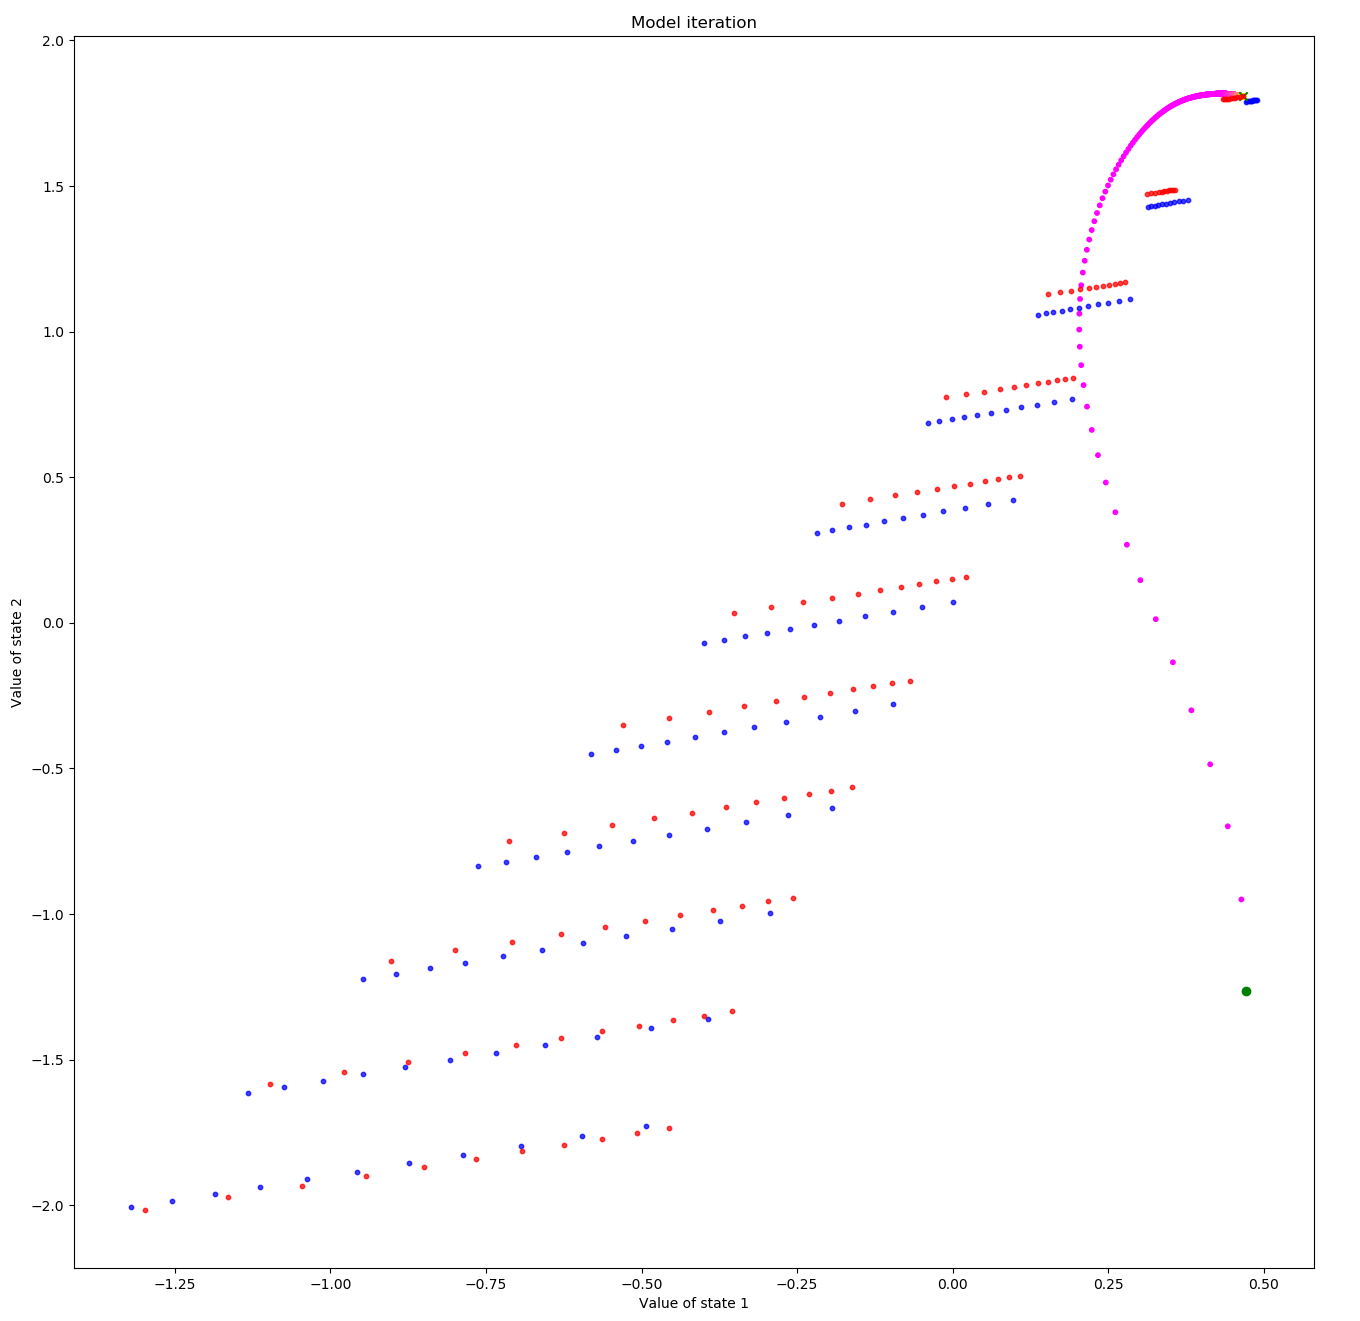
\includegraphics[width=0.5\textwidth,height=0.5\textheight]{../../pictures/figures/model_iteration.png}
\caption{Blue shows the value of policies when evaluated under the true model, $P, r$,
and Red shows the estimated value of policies when evaluated under the learned model at convergence, $\tilde P, \tilde r$.}
\end{figure}


Related to AWR? https://arxiv.org/pdf/1910.00177.pdf

\subsubsection{Compressed sensing}

words



\begin{center}\rule{0.5\linewidth}{\linethickness}\end{center}

So there seem to be three different classes of search space: each imbued with special
structure from the Bellman equation. Each with different the types of search they
support. And each with different parameter topologies.

What are their properties? And which spaces support efficient search for the optimal policy?

\begin{itemize}
\tightlist
\item
  In the value space we can use the temporal difference operator,
\item
  in the policy space we can estimate policy gradients,
\item
  in the model space we can solve directly for the optimal policy.
\end{itemize}

\section{Gradient based search}

% need a better seguae into GD?!
Let's focus on searching with gradient descent.

\begin{align}
w_{t+1} = w_t - \eta \nabla f(w_t)
\end{align}

The dynamics of the search are dependent on the topology of a problems loss surface.
The loss surface is determined by the combination of the search space and the loss function.

\subsection{Parameterised search}

\begin{align}
&\mathop{\text{max}}_V \mathop{\mathbb E}_{s\sim D} V(s) \\
&\mathop{\text{max}}_{\pi} \mathop{\mathbb E}_{s\sim D}V^{\pi}(s) \\
&\mathop{\text{max}}_{\theta} \mathop{\mathbb E}_{s\sim D} V_{\theta}(s)\label{eq:deepQ}\\
&\mathop{\text{max}}_{\theta} \mathop{\mathbb E}_{s\sim D} V^{\pi_{_{\theta}}}(s) \\
&\mathop{\text{max}}_{\theta} \mathop{\mathbb E}_{s\sim D} V_{\theta}^{\pi_{_{\phi}}}(s)\label{eq:actorcritic} \\
&\mathop{\text{max}}_{\phi} \mathop{\mathbb E}_{s\sim D} V^{\pi_{_{\theta_{\phi}}}}(s)
\end{align}

Value iteration and related methods like (deep) Q learning. \eqref{eq:deepQ}
\eqref{eq:actorcritic}

Ok. So when $\phi$ are the parameters of a deep neural network, ...? The search space has certain (which) properties.
Euclidean geometry.
(parameter dimensions are independent! no funny business)

We can pick any space we we like to search with in. But, why would we want to pick one space over another?
What properties are we looking for?

\begin{itemize}
\tightlist
\item
  In which spaces can we (efficiently) calculate gradients?
\item
  In which spaces can we do convex optimisation?
\item
  In which spaces does momentum work (well)?
\end{itemize}


\subsection{Dynamics and complexity}

\begin{displayquote}
  \textit{So. We want to investigate the properties of gradient based search in different search spaces.}
\end{displayquote}

Let start with trying to understand the different dynamics and iteration complexities.

How can you quantify a trajectory?

What about the vector fields?
Do some spaces have gradients that most globally point in approximately the right direction?



\begin{figure}
\centering
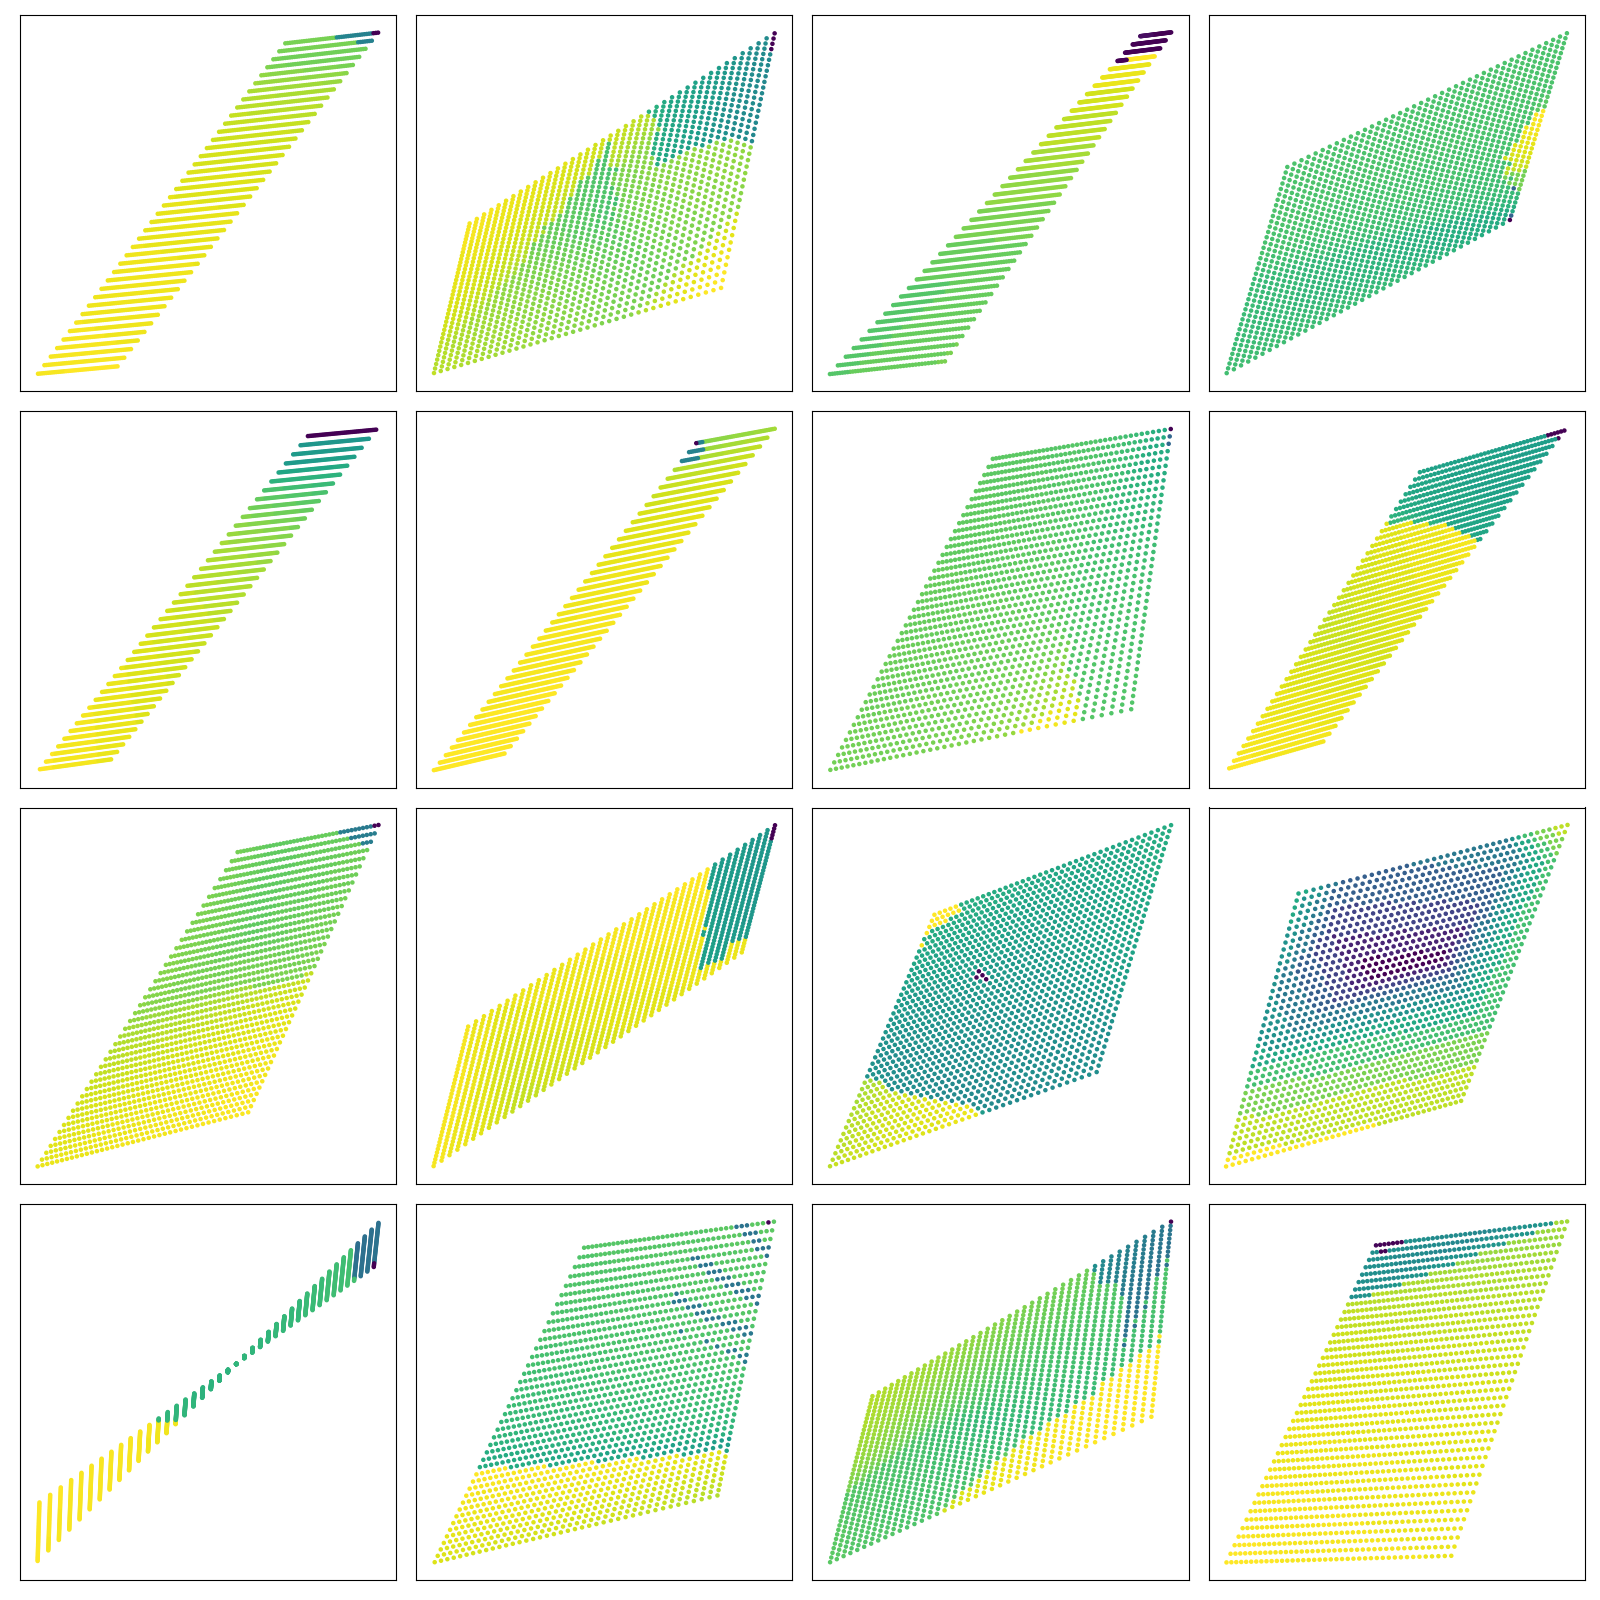
\includegraphics[width=1\textwidth,height=1\textheight]{../../pictures/figures/mvi-iterations.png}
\caption{Above you see: various MDPs where the value of each policy is colored
by the number of iterations it took to converge to the optimum policy. Yellow is many iterations, purple is few iterations.}
\end{figure}

\begin{itemize}
\tightlist
\item
  What are the best ways to travel through policy space? (lines of
  shortest distance?!)
\item
  How does this scale with \texttt{n\_actions} or \texttt{n\_states}??
\item
  Is there a way to use an interior search to give info about the
  exterior? (dual methods?!)
\item
  What if your evaluations are only \(\epsilon\)-accurate? How does that
  effect things?!?
\item
  how can we pick the topology for better dynamics!?
\end{itemize}



%  include iteration plots

The momentum polts tell us that if we want to bound the iteration complexity of GD plus momentum
then ...? We need a term that caputures the position / oscillation dynamics!?
% TODO want a better picture of the difference between these trajectories.


\subsection{Acceleration and parameterisation}

I think something weird happens with momentum in overparameterised spaces. The intuition is

\cite{Arora2018} shows that overparameterisation yields acceleration. Consider
the dynamics of the parameter $w$, which we have overparameterised as $w_1 \cdot w_2$.

\begin{align}
w^{t+1} &= w_1^{t+1} \cdot w_2^{t+1} \\
&= (w_1^t - \eta \nabla_{w_1} L)\cdot(w_2^t - \eta \nabla_{w_2} L) \\
&= (w_1^t \cdot w_2^t - \eta w_2^t \nabla_{w_1} L - \eta w_1^t \nabla_{w_2} L - \mathcal O(\eta^2) \\
&= w^t - ...
\end{align}

We have implicit momentum from the parameterisation, and explicit momentum in the accelerated descent.


\begin{align}
m_{t+1} &= \gamma m_t + g_t \\
w_{t+1} &= w_t - \eta \cdot (1-\gamma) \cdot m_t
\end{align}

It is necessary to consider the trajectory to study momentum. It depends
on what has happened in the past. Can we construct a space of possible
trajectories? What properties do trajectories have? They are connected
by the update fn.


\section{Topology and dynamics}

What kinds of query and movement does our search space support?

If we parameterise our search space. We my have changed the topology of our search space.
Is it possible to arbitrarily change the topology? (probably?!?)

\textbf{Q:} How can we rationally pick the topology of our search space
to accelerate learning?

\begin{itemize}
\item
  A well connected space? For all possible policies, there exists
  \(\theta_1, \theta_2 \text{ s.t. } \parallel \theta_1- \theta_2\parallel_2\)
  is small. (but that doesnt necessarily help\ldots{} depends on the
  landscapce imposed by \(\nabla_{\theta} V\))
\item
  ???
\end{itemize}

See these gradient flows for example;

Pics?!?

Here are some examples \ldots{}???

\begin{figure}
\centering
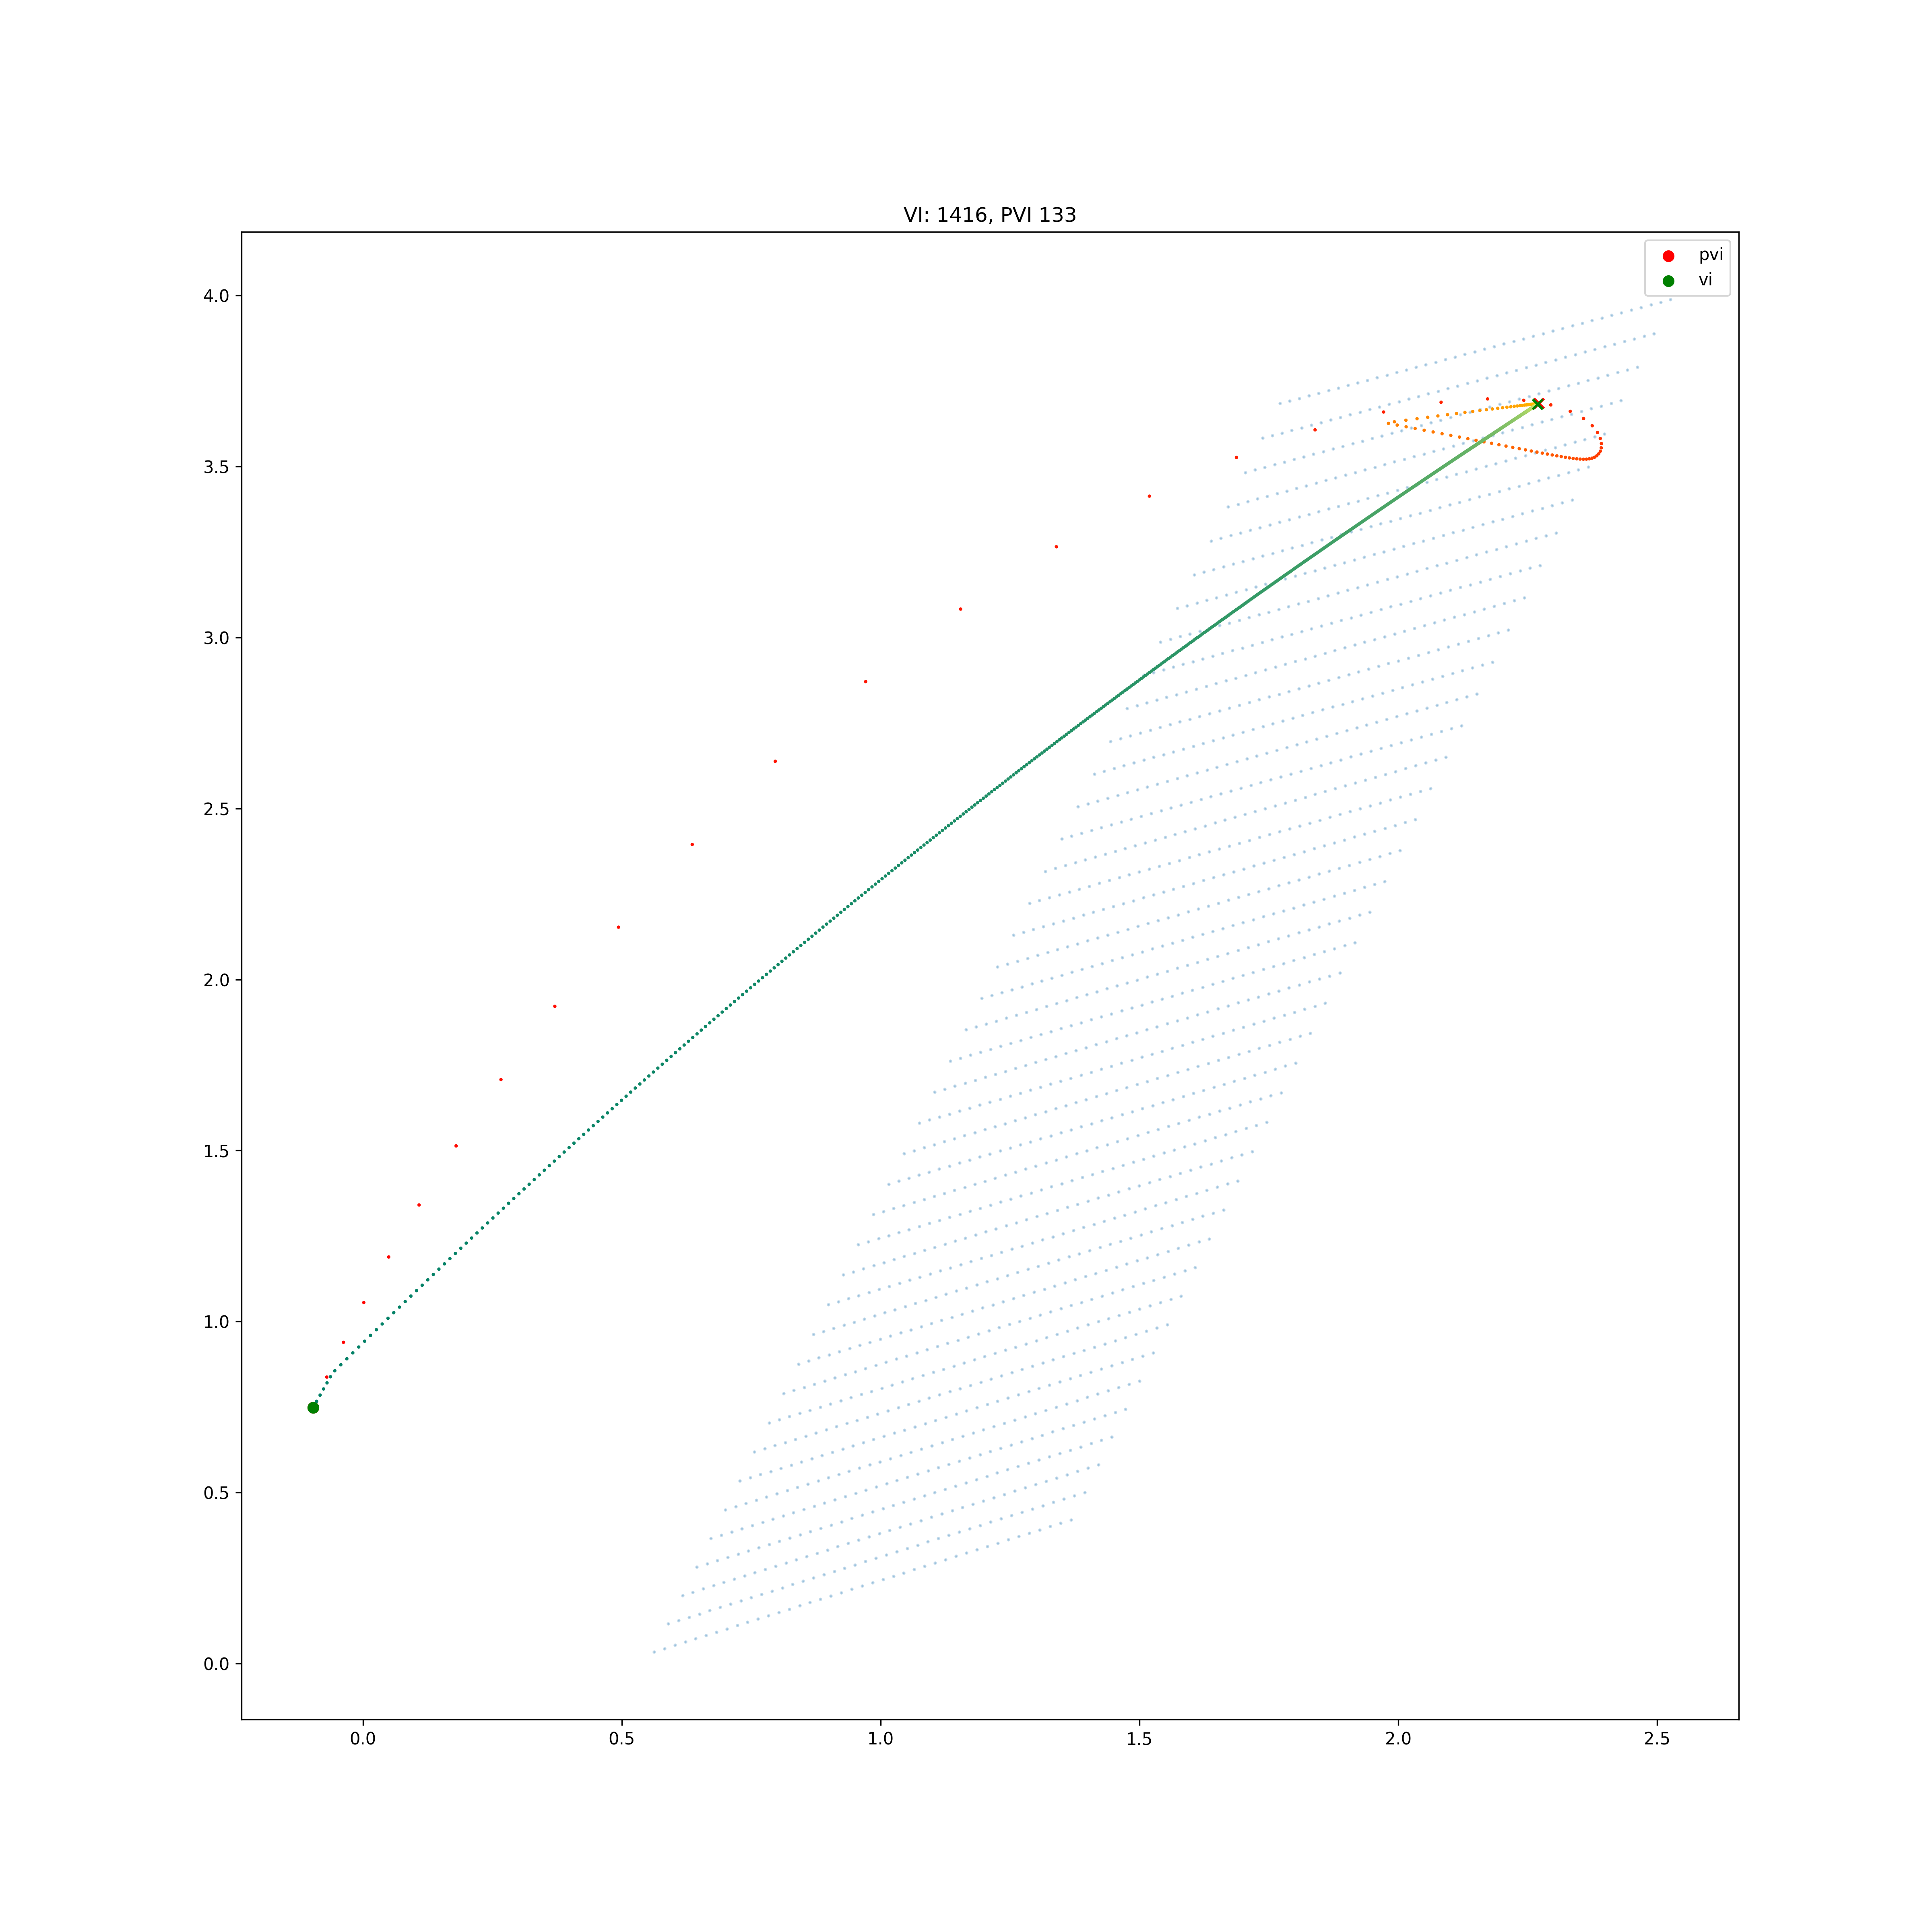
\includegraphics[width=0.5\textwidth,height=0.5\textheight]{../../pictures/figures/vi-vs-pvi.png}
\caption{The optimisation dynamics of value iteration versus parameterised value iteration.}
\end{figure}

\begin{figure}
\centering
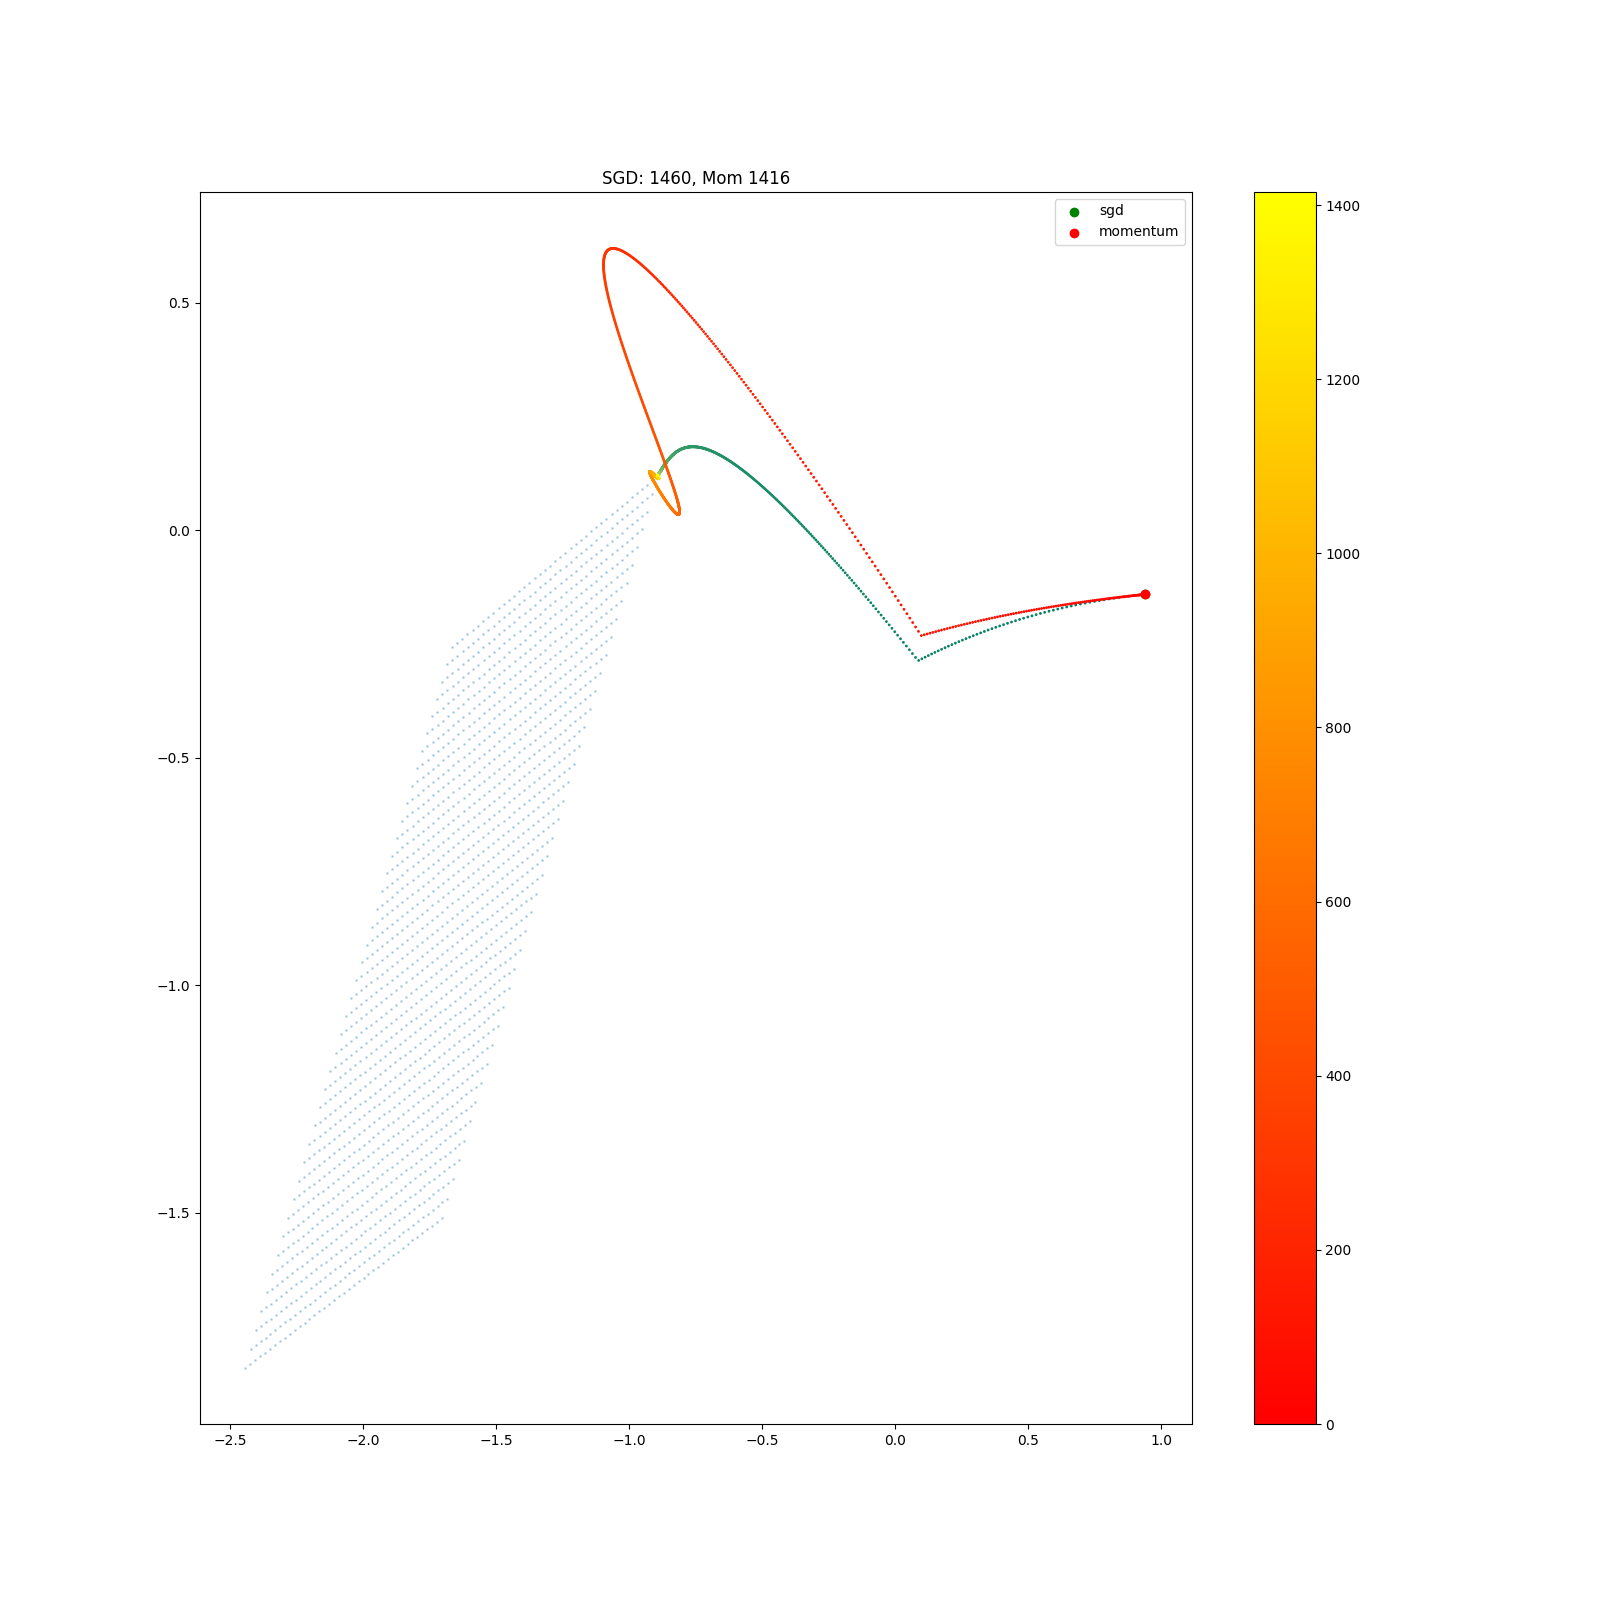
\includegraphics[width=0.5\textwidth,height=0.5\textheight]{../../pictures/figures/vi_sgd-vs-vi_mom.png}
\caption{The optimisation dynamics of value iteration versus value iteration with momentum.}
\end{figure}

If we overparameterise the search space, then we can move between solutions in new ways. We can `tunnel' from A to B, without crossing C.
%  insert pic / prove

Every point (in output space) is closer, when measured in the distance in parameter space needed to be traveled.
% insert pic / prove


\section{Continuous flow and its discretisation}

A linear step of size, \(\alpha\), in parameter space, ie by gradient
descent, is not necessrily a linear step in parameter space.

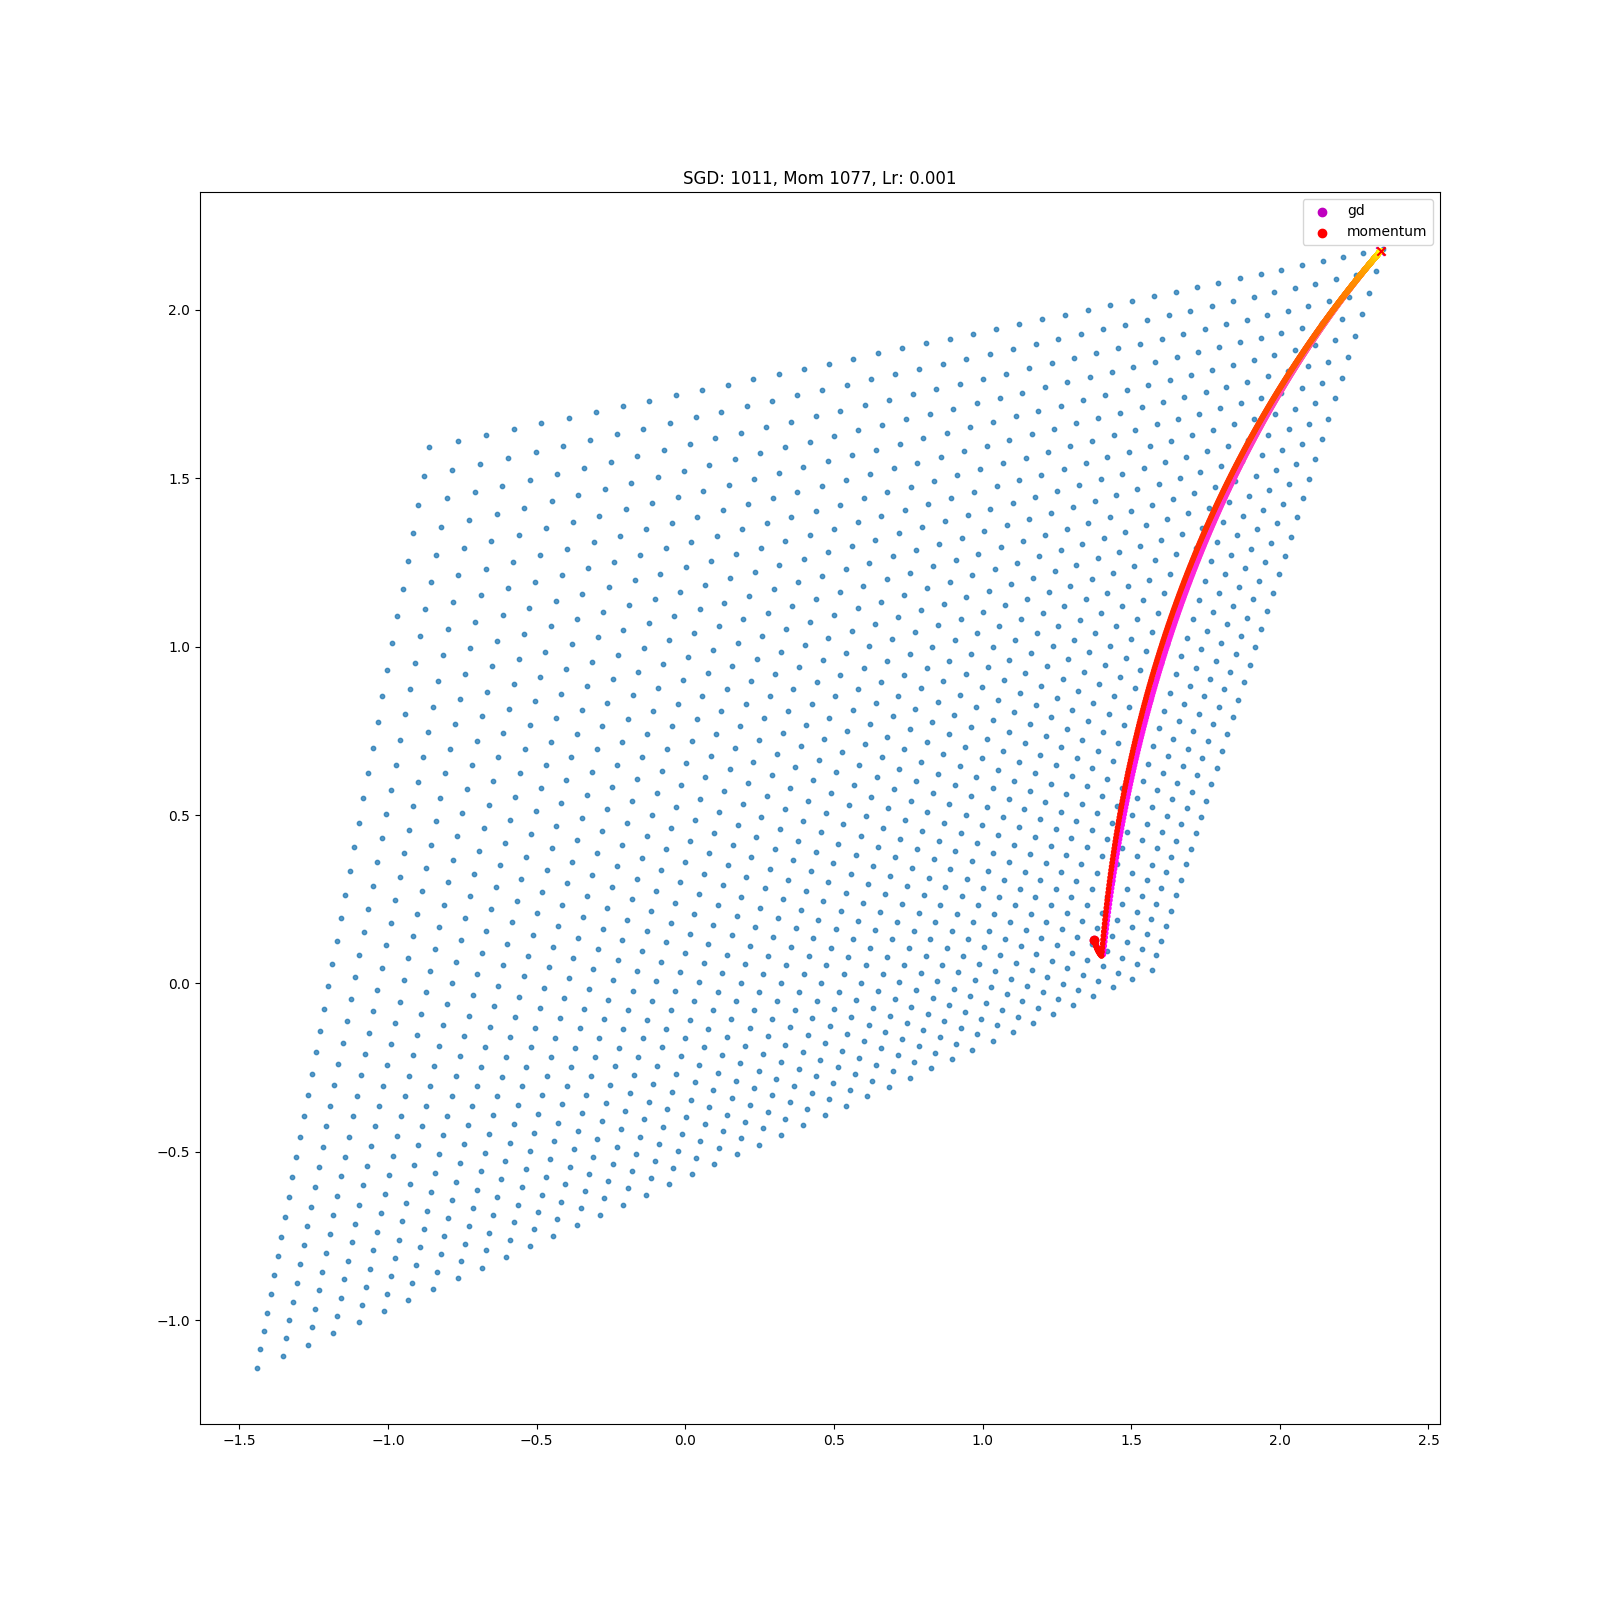
\includegraphics[width=0.3\textwidth,height=0.25\textheight]{../../pictures/figures/vi_sgd-vs-vi_mom_0001.png}
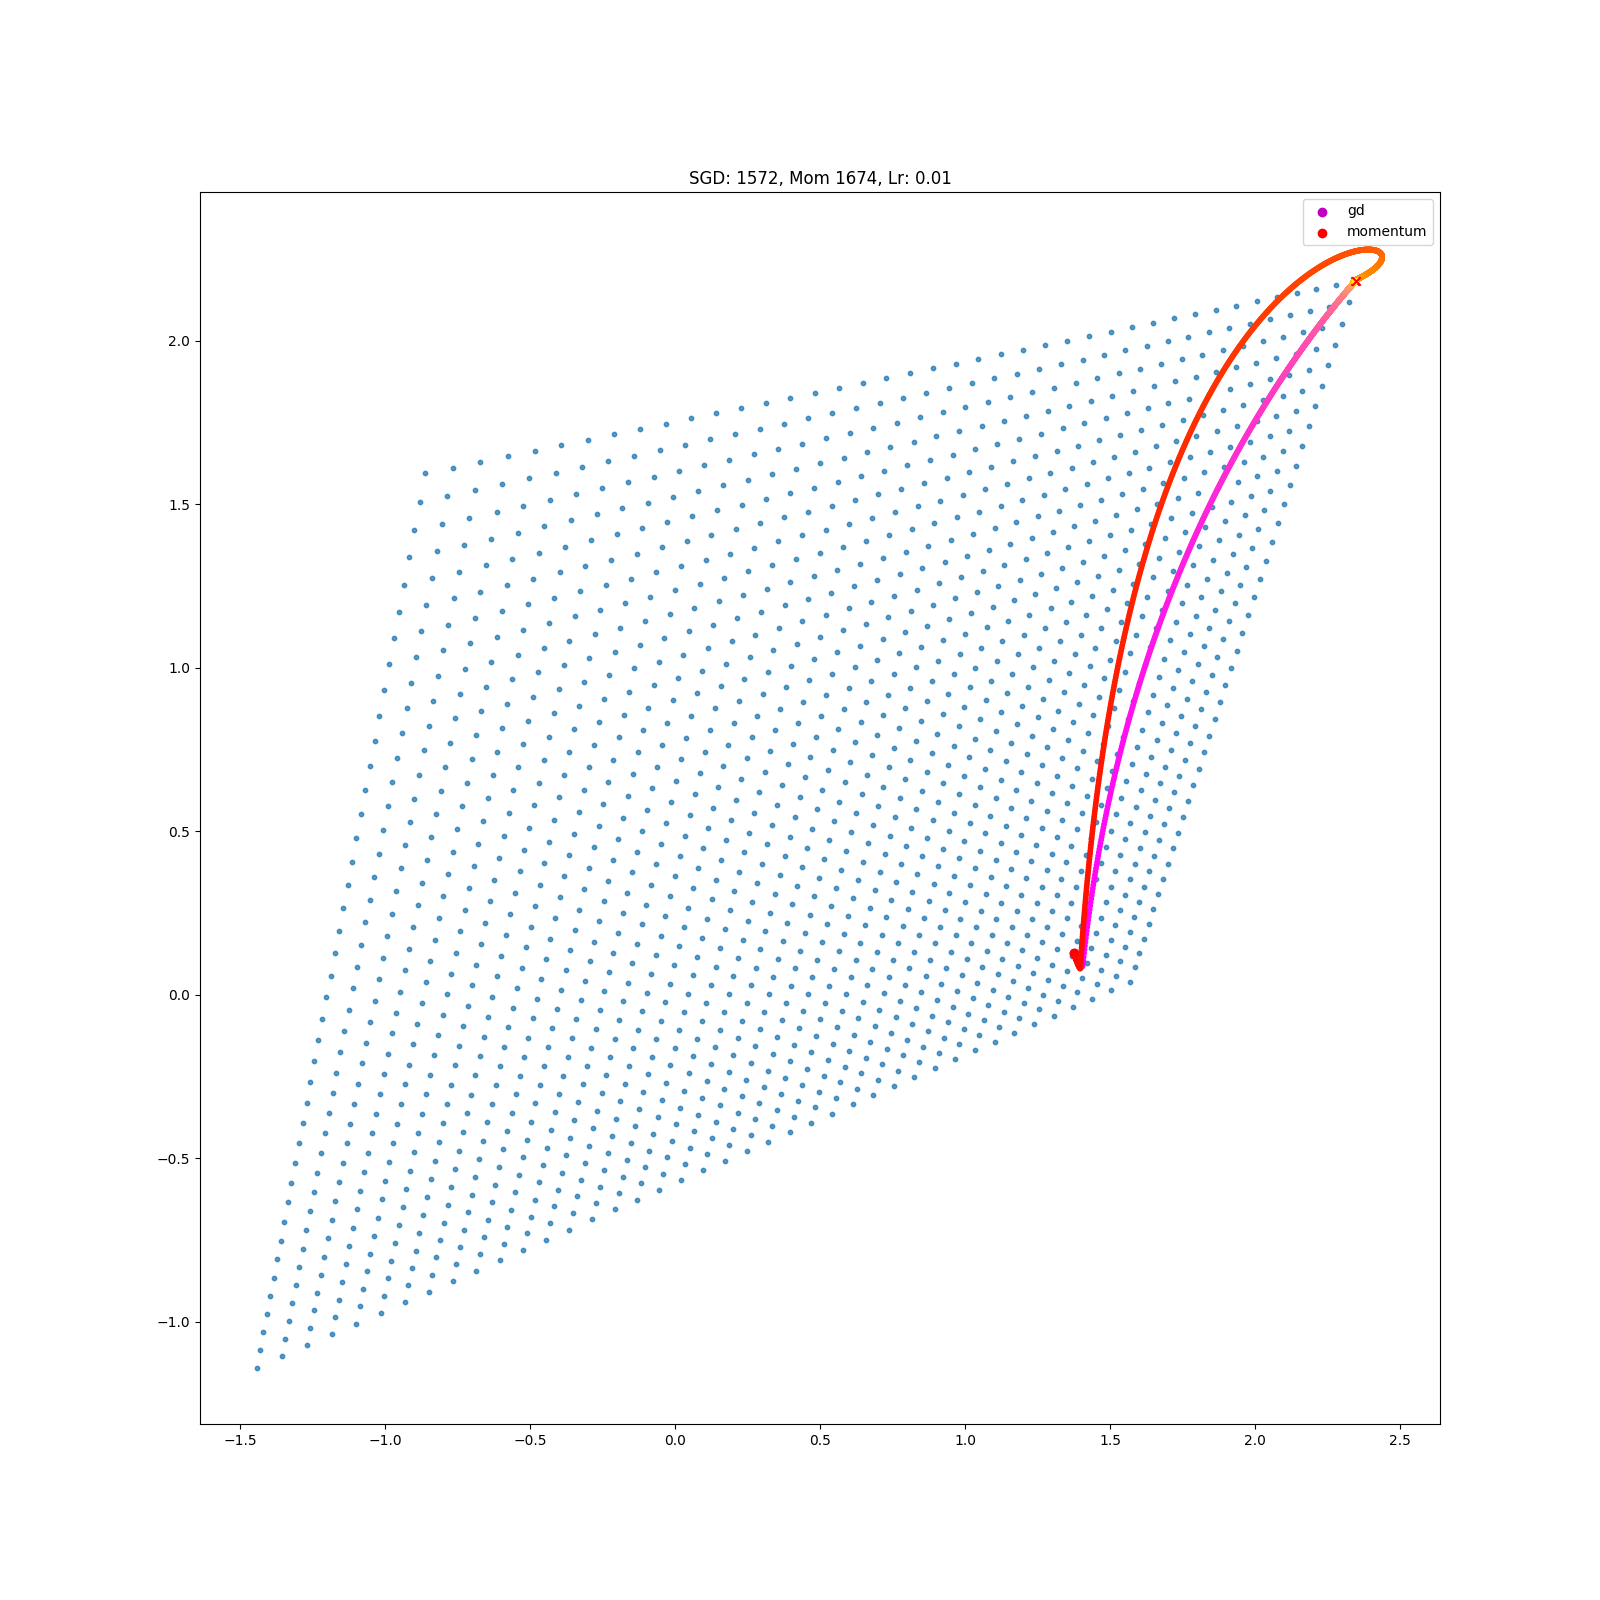
\includegraphics[width=0.3\textwidth,height=0.25\textheight]{../../pictures/figures/vi_sgd-vs-vi_mom_001.png}
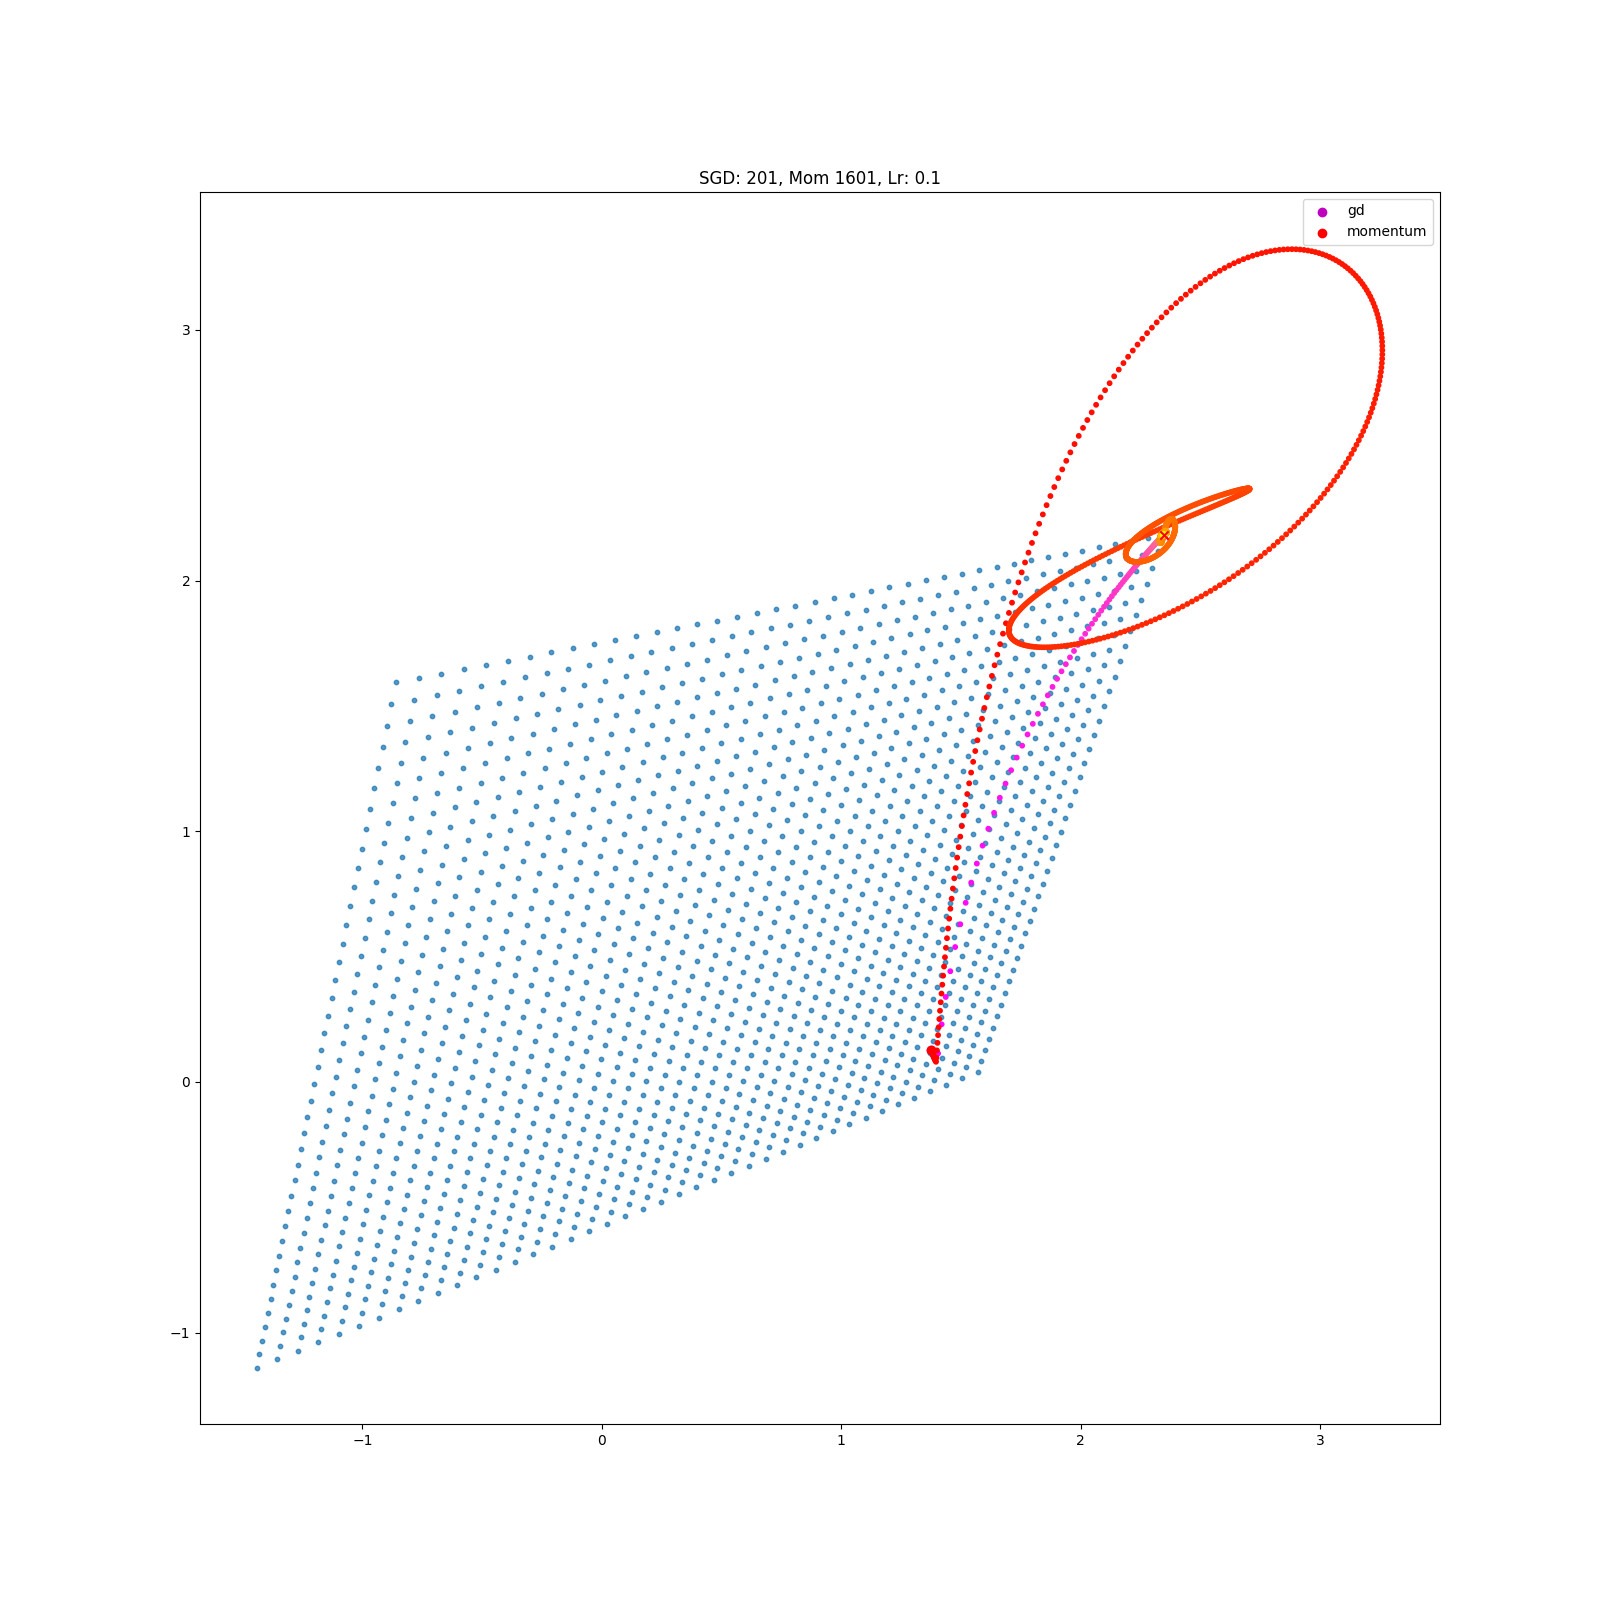
\includegraphics[width=0.3\textwidth,height=0.25\textheight]{../../pictures/figures/vi_sgd-vs-vi_mom_01.png}

This is consistent with acceleration of gradient descent being a phenomena only possible in the discrete time setting. (see \cite{Betancourt2018} for a recent exploration)

This phenomena can be explained by the exponential decay of the momentum terms.

\begin{align}
m_{t+1} = m_t + \gamma\nabla f(w_t) \\
w_{t+1} = w_t - \eta (1-\gamma) m_{t+1} \\
\end{align}

As \(\eta \to 0\), \((1-\gamma) \cdot m_{t+1} \to \nabla f(w_t)\).

TODO, prove it.

\section{Notes}

When transforming between two spaces, how does the optimisation space
change? Does my abstraction make optimisation easier?


\section{Related work}

Recently there has been work investigating the properties of overparameterised search spaces.
Many \cite{Arora2018} (and others?!?!?) claim that overparameterisation yeilds acceleration, however,
their explanation of the acceleration is not entirely convincing. Bc...

How does momentum bias the kinds of solution that is converged to. (not really a question for RL?!)
Do we care aout the intermediate policies? In the synchronous setting no. In the asynchronous setting yes.
How does momentum bias trajectories? To cover more distance? To have more diversity?

Search spaces with alternative geometries.
Hyperbolic neural networks. https://arxiv.org/pdf/1805.09112.pdf
